\begin{titlepage}
\begin{center}

\includegraphics[scale=0.15]{OPAMP Config/niser.png}
\line(1,0){400}\\
[2mm]
\begin{large}
\textbf{\huge Study of Basic Op-Amp Configurations}\\ 
\end{large}
\line(1,0){250}\\
[5cm]
\large MAITREY SHARMA\\
\small (1911093)\\
[4.5cm]
Second Year Integrated M.Sc.\\
\textbf{School of Physical Sciences}\\
\textbf{National Institute of Science Education and Research, Bhubaneshwar}\\
\small March 3, 2021
\end{center} 
\end{titlepage}
\newpage
\section{Aim}
\begin{itemize}
    \item Study of the inverting amplifier configuration and to find its gain
    \item Study of the non-inverting amplifier configuration and to find its gain
    \item Study simple mathematical operation and design an averaging amplifier
\end{itemize}
\section{Apparatus}
\noindent Op-Amp IC741, resistors, oscilloscope, DC voltage source, breadboard.
\section{Theory}
\noindent \textbf{\emph{Operational Amplifiers}} or \textbf{\emph{Op-Amps}} are linear devices having properties required for DC amplification and are used in conditioning, filtering or to perform mathematical operations such as addition, subtraction, differentiation and integration.
\newline The most widely available Op-Amp is the industry standard IC741 as shown below.
\begin{center}
    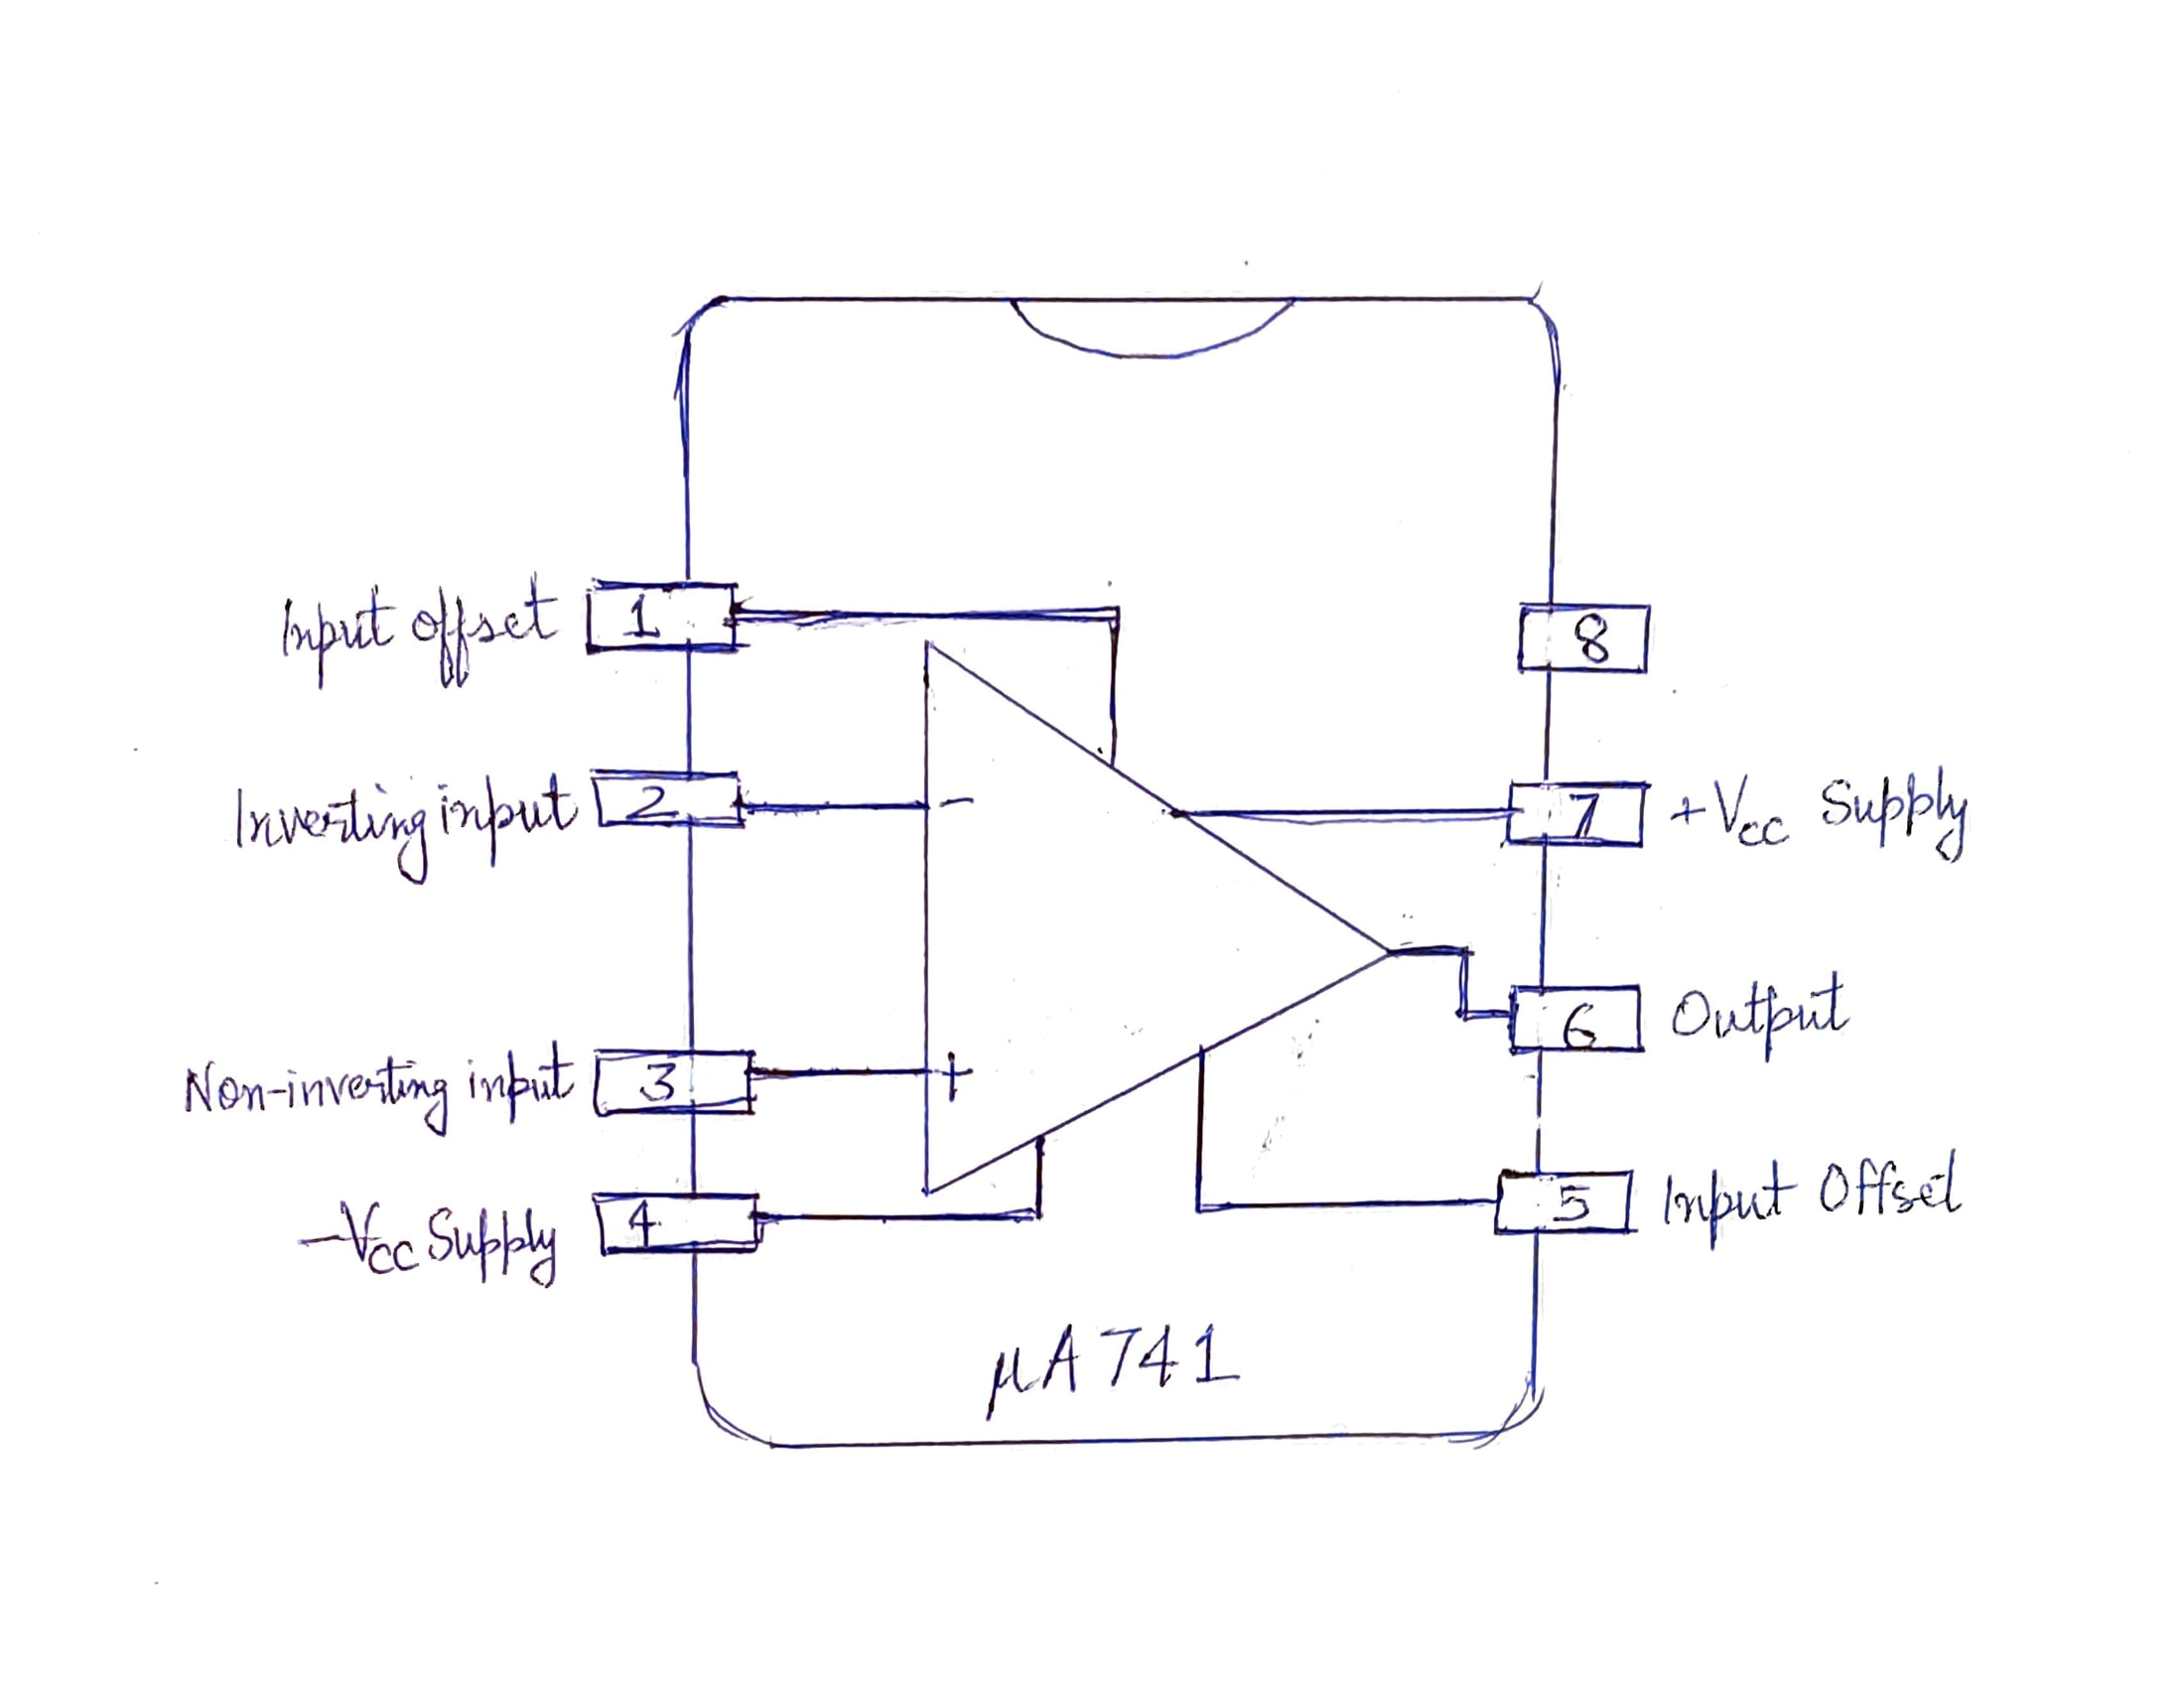
\includegraphics[scale = 0.15]{OPAMP Config/IC741.jpg}
\end{center}
\noindent There are several types of circuits that can be constructed depending on the usage of the Op-Amp. In absence of any feedback, that is, the case of open loop, the gain is very high (ideally infinite). To evade this, we can connect a suitable resistor from the output terminal back to the inverting input terminal, thus creating a negative feedback which results in the formation of a very stable Op-Amp system. This type of Op-Amp is called an \textbf{\emph{Inverting Amplifier}} as depicted in the circuit diagram on the next page.
\clearpage
\begin{center}
    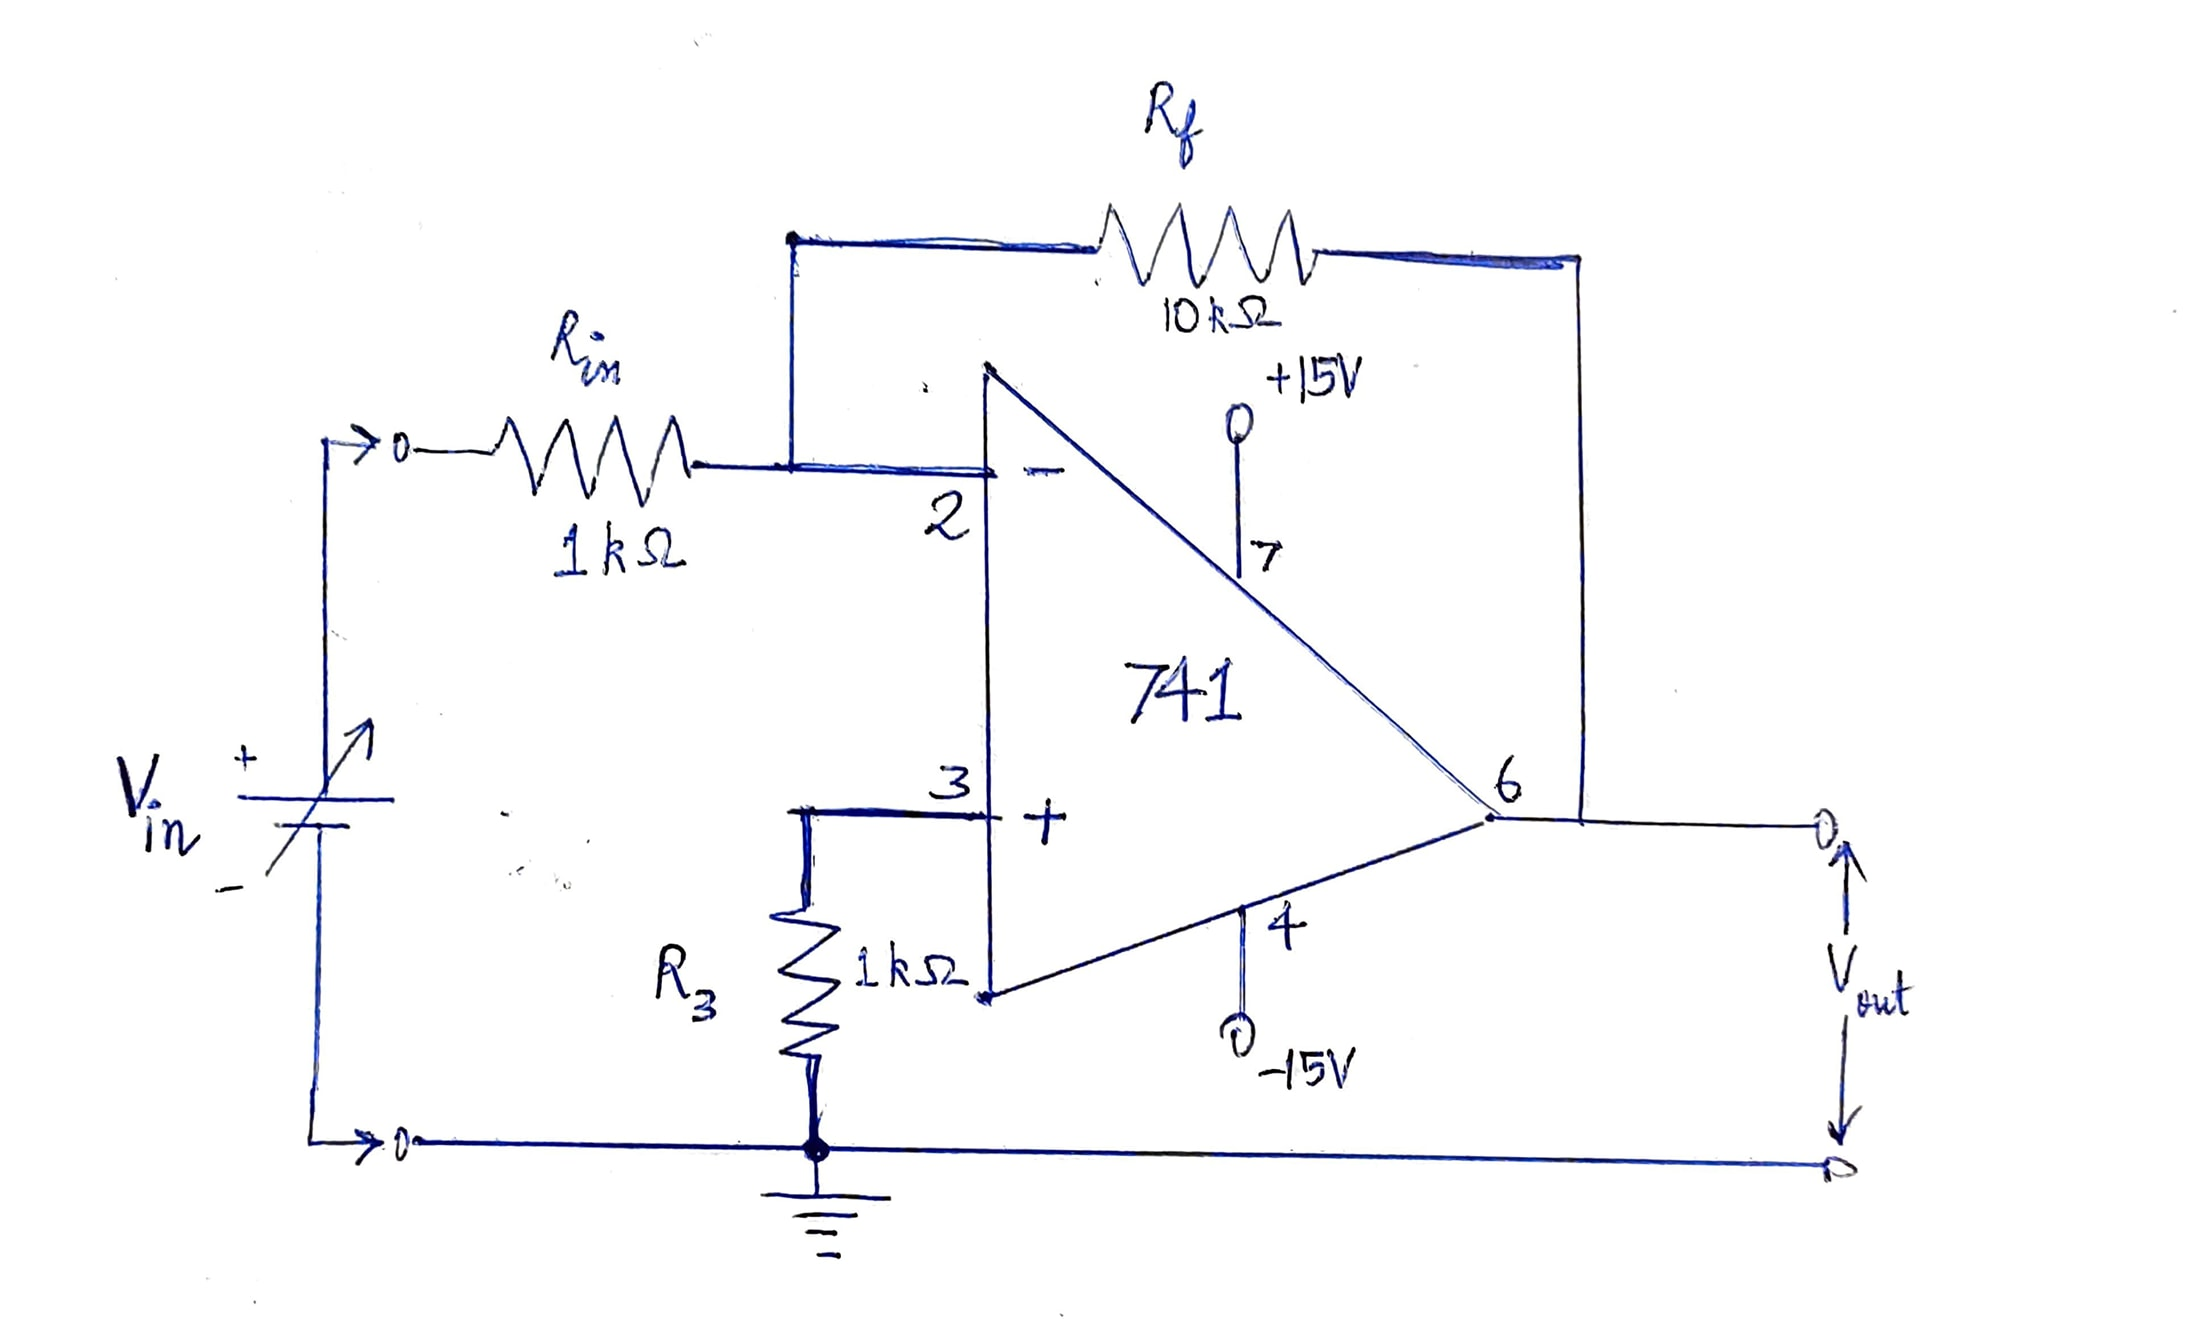
\includegraphics[scale = 0.15]{OPAMP Config/inv.jpg}
\end{center}
\begin{center}
    \textbf{Inverting Amplifier Circuit}
\end{center}
The formula to calculate the \textbf{\emph{Gain}} in this case is:
\begin{center}
    Gain, $A = \dfrac{V_o}{V_{i}} = -\dfrac{R_f}{R_i}$
\end{center}
Similarly, if the output terminal is connected back to the non-inverting input terminal, again a negative feedback is generated but with a positive gain this time. This type of Op-Amp is called \textbf{\emph{Non-inverting Amplifier}}.
\begin{center}
    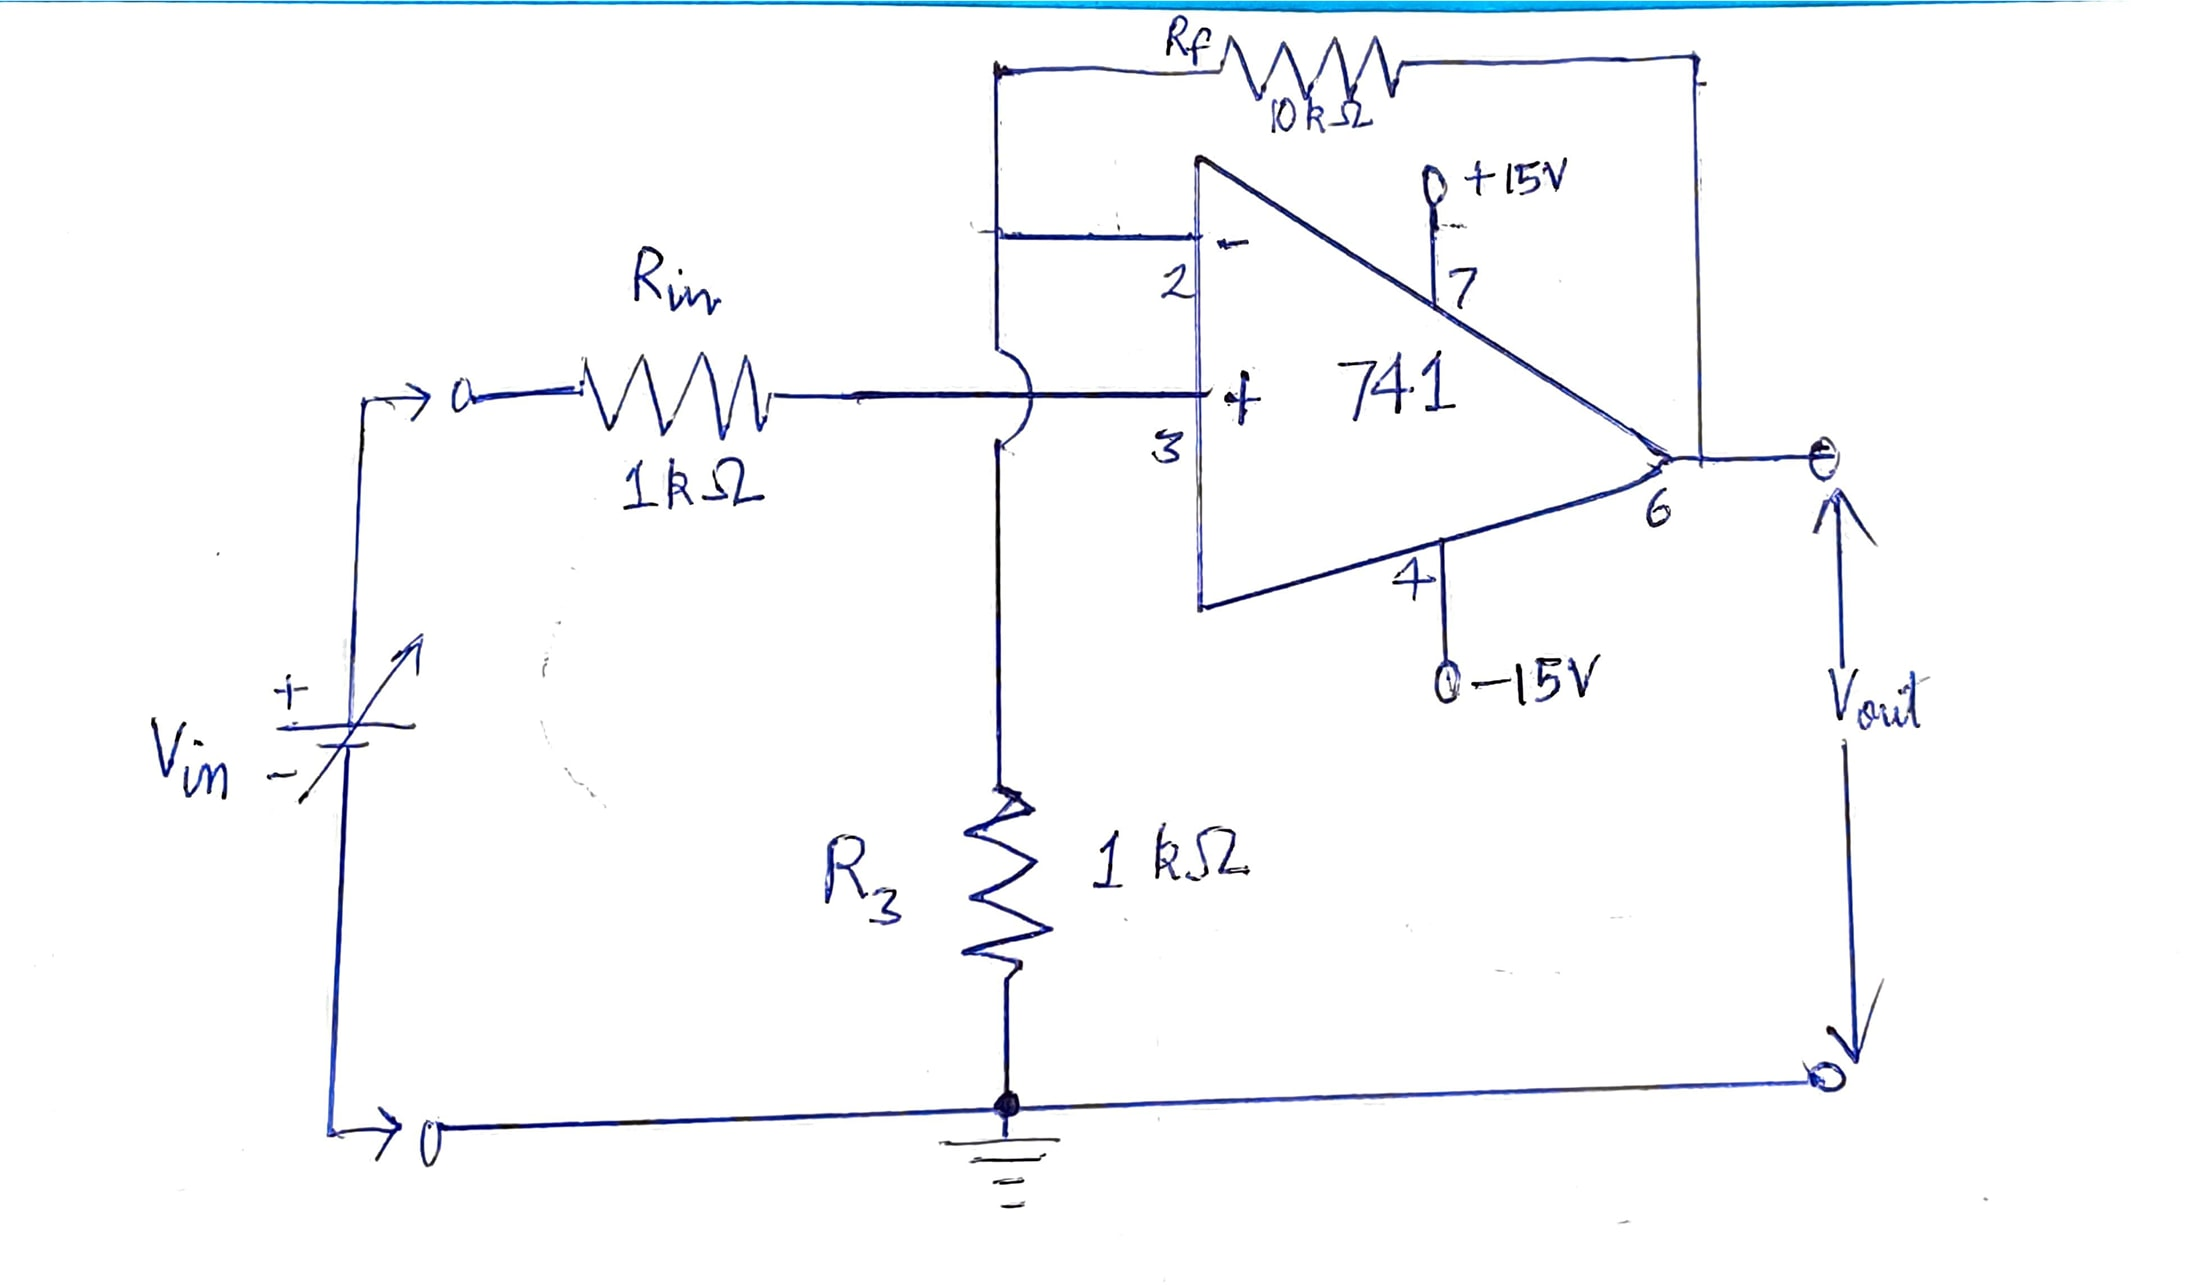
\includegraphics[scale = 0.15]{OPAMP Config/noninv.jpg}
\end{center}
\begin{center}
    \textbf{Non-Inverting Amplifier Circuit}
\end{center}
\clearpage
\noindent Here, 
\begin{center}
    Gain, $A = \dfrac{V_o}{V_{i}} = 1 + \dfrac{R_f}{R_i}$
\end{center}
Using the inverting amplifier we can also create a \textbf{\emph{Summing Amplifier}} circuit, in which the output voltage is proportional to the summation of all the input voltages and the constant of proportionality being the \textbf{\emph{Gain}} of the circuit.
\begin{center}
    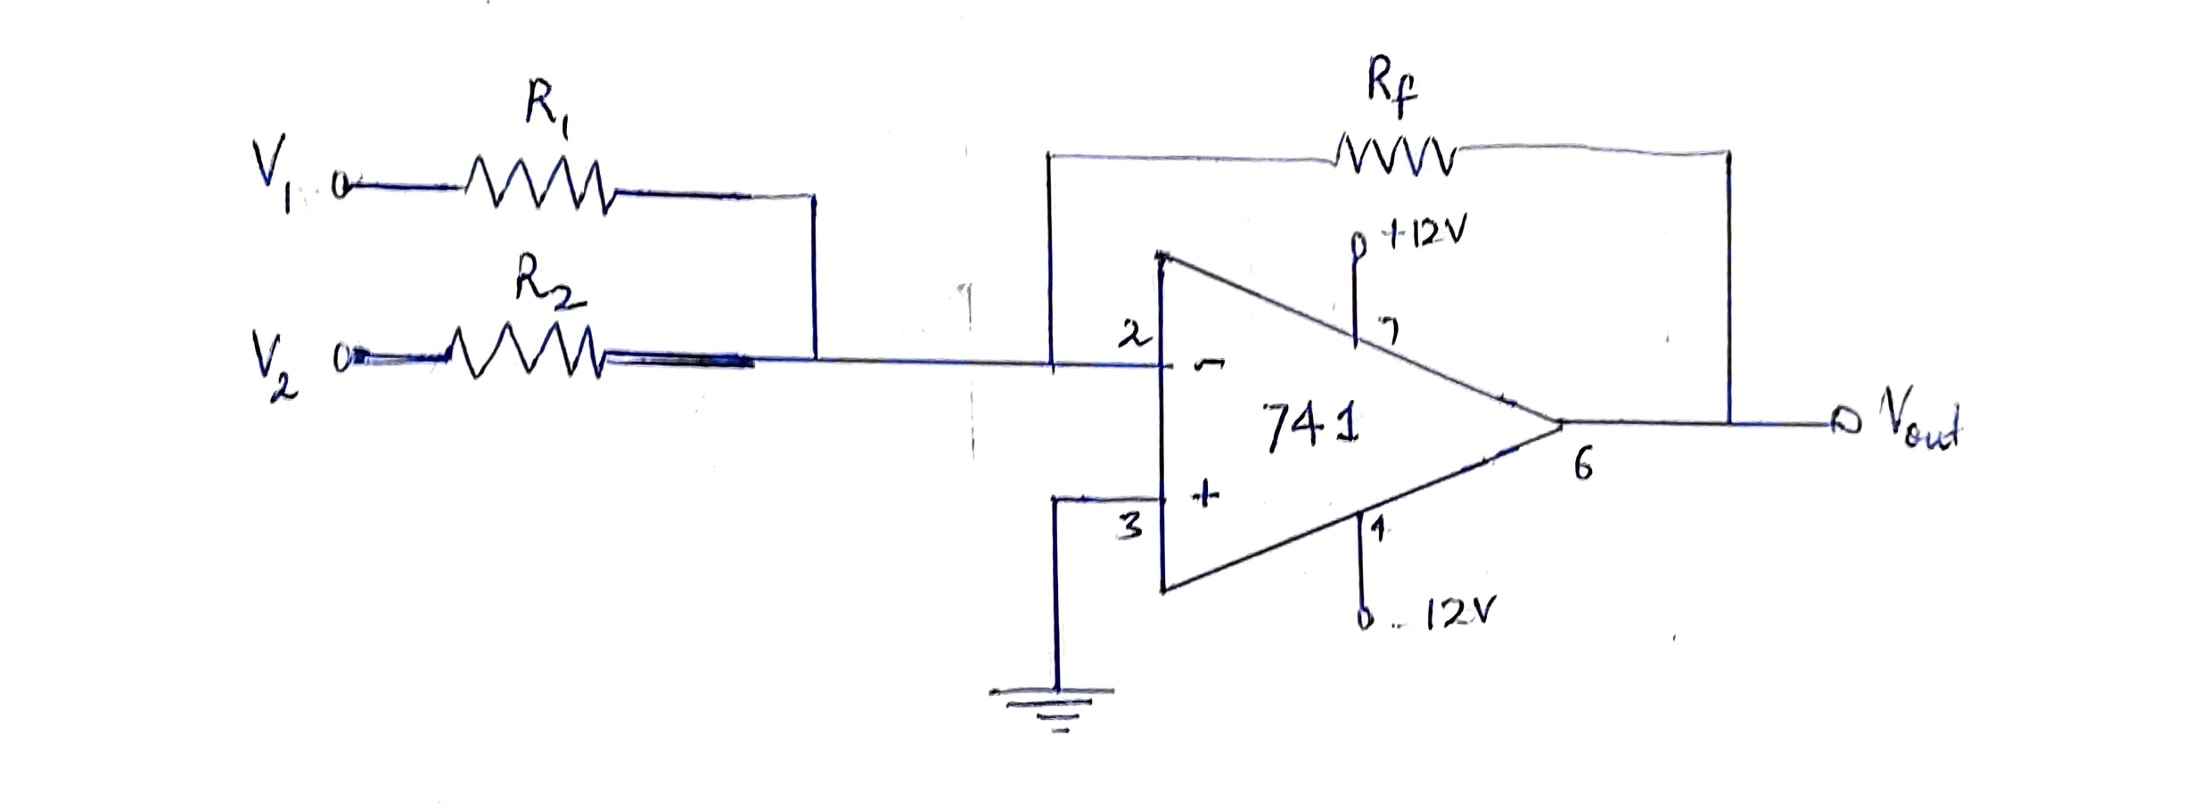
\includegraphics[scale = 0.2]{OPAMP Config/summing.jpg}
\end{center}
\begin{center}
    \textbf{Summing Amplifier Circuit}
\end{center}
\noindent The relation between the circuit components can be written as: 
\begin{center}
    $V_o = - \dfrac{R_f}{R_i}(V_1 + V_2)$
\end{center}
In the same way, we can also create a \textbf{\emph{Difference Amplifier}} circuit by connecting input voltages to both inverting and non-inverting input terminals at the same time. The resultant output voltage would be proportional to the difference of the input voltages this time.
\begin{center}
    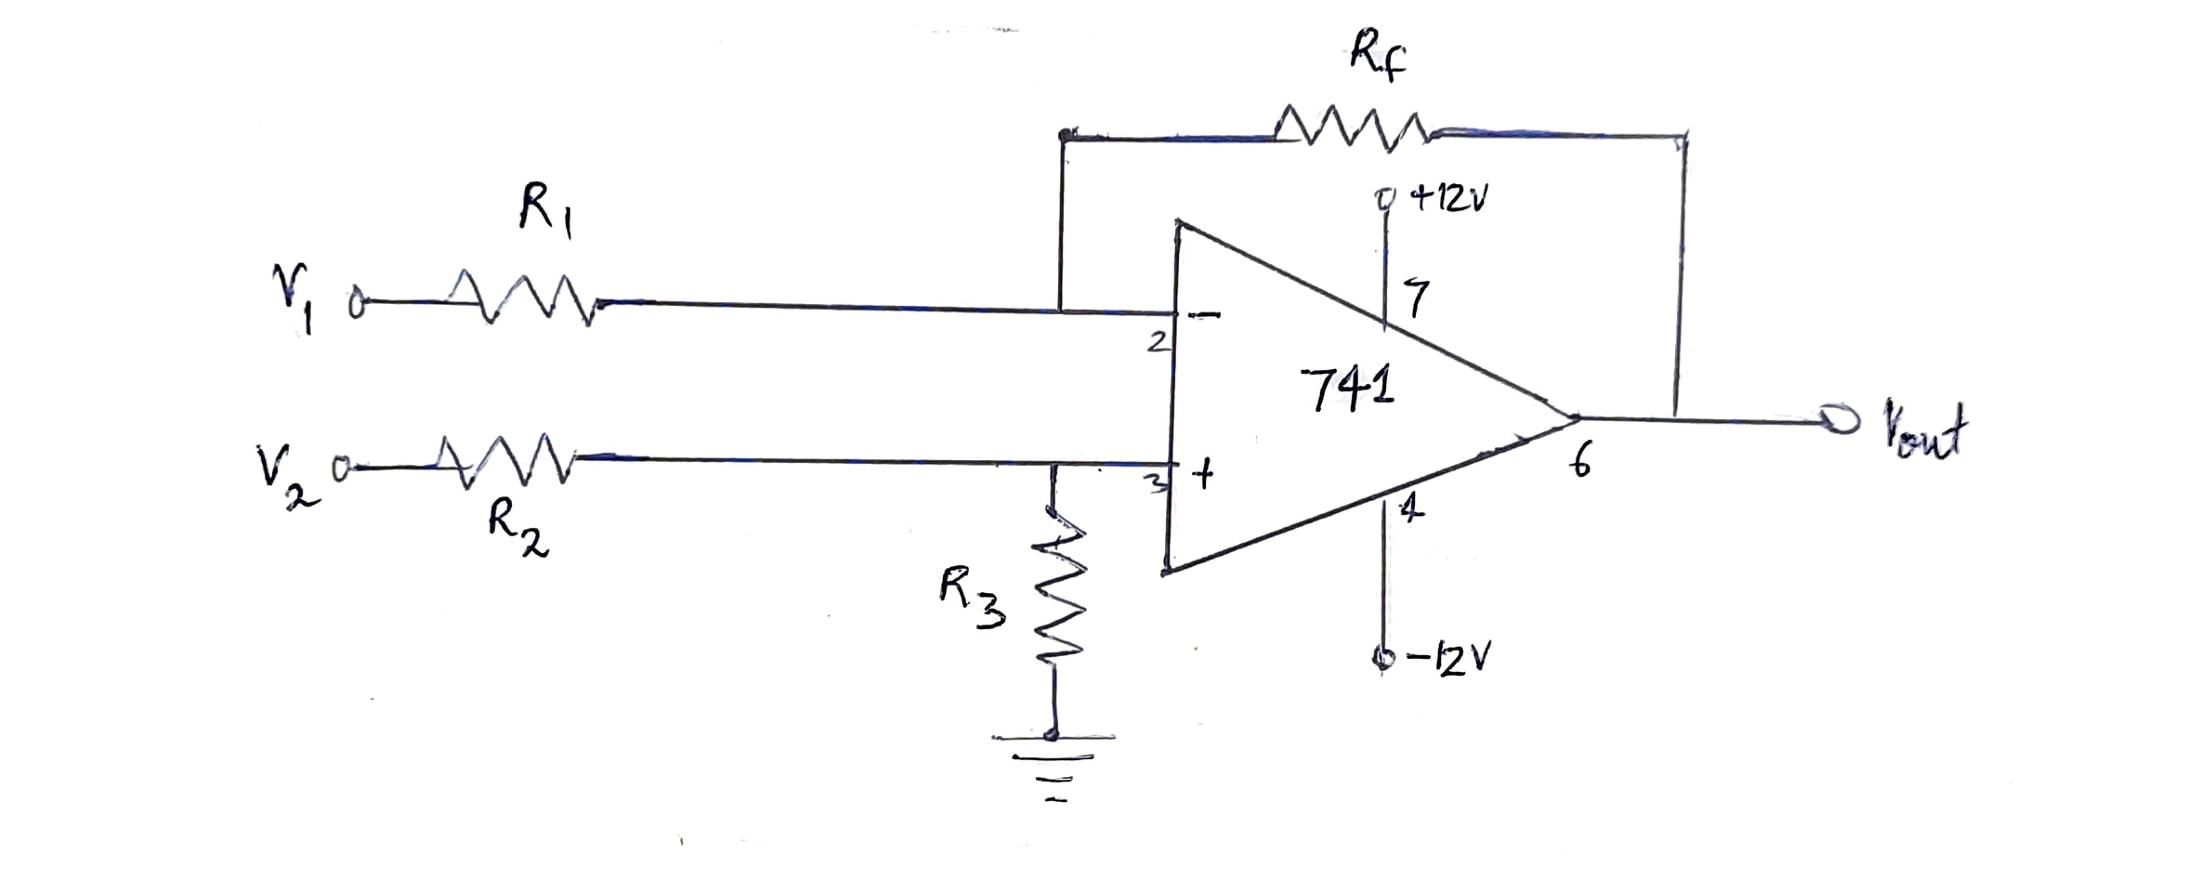
\includegraphics[scale = 0.18]{OPAMP Config/difference.jpg}
\end{center}
\begin{center}
    \textbf{Difference Amplifier Circuit}
\end{center}
\noindent The relation in this case becomes:
\begin{center}
    $V_o = - \dfrac{R_f}{R_i}(V_1 - V_2)$
\end{center}

Lastly, we can design one more configuration using the inverting amplifier case. As seen from the formulae, by halving the feedback resistor $R_f$, we can construct an \textbf{\emph{Averaging Amplifier}} circuit.
\begin{center}
    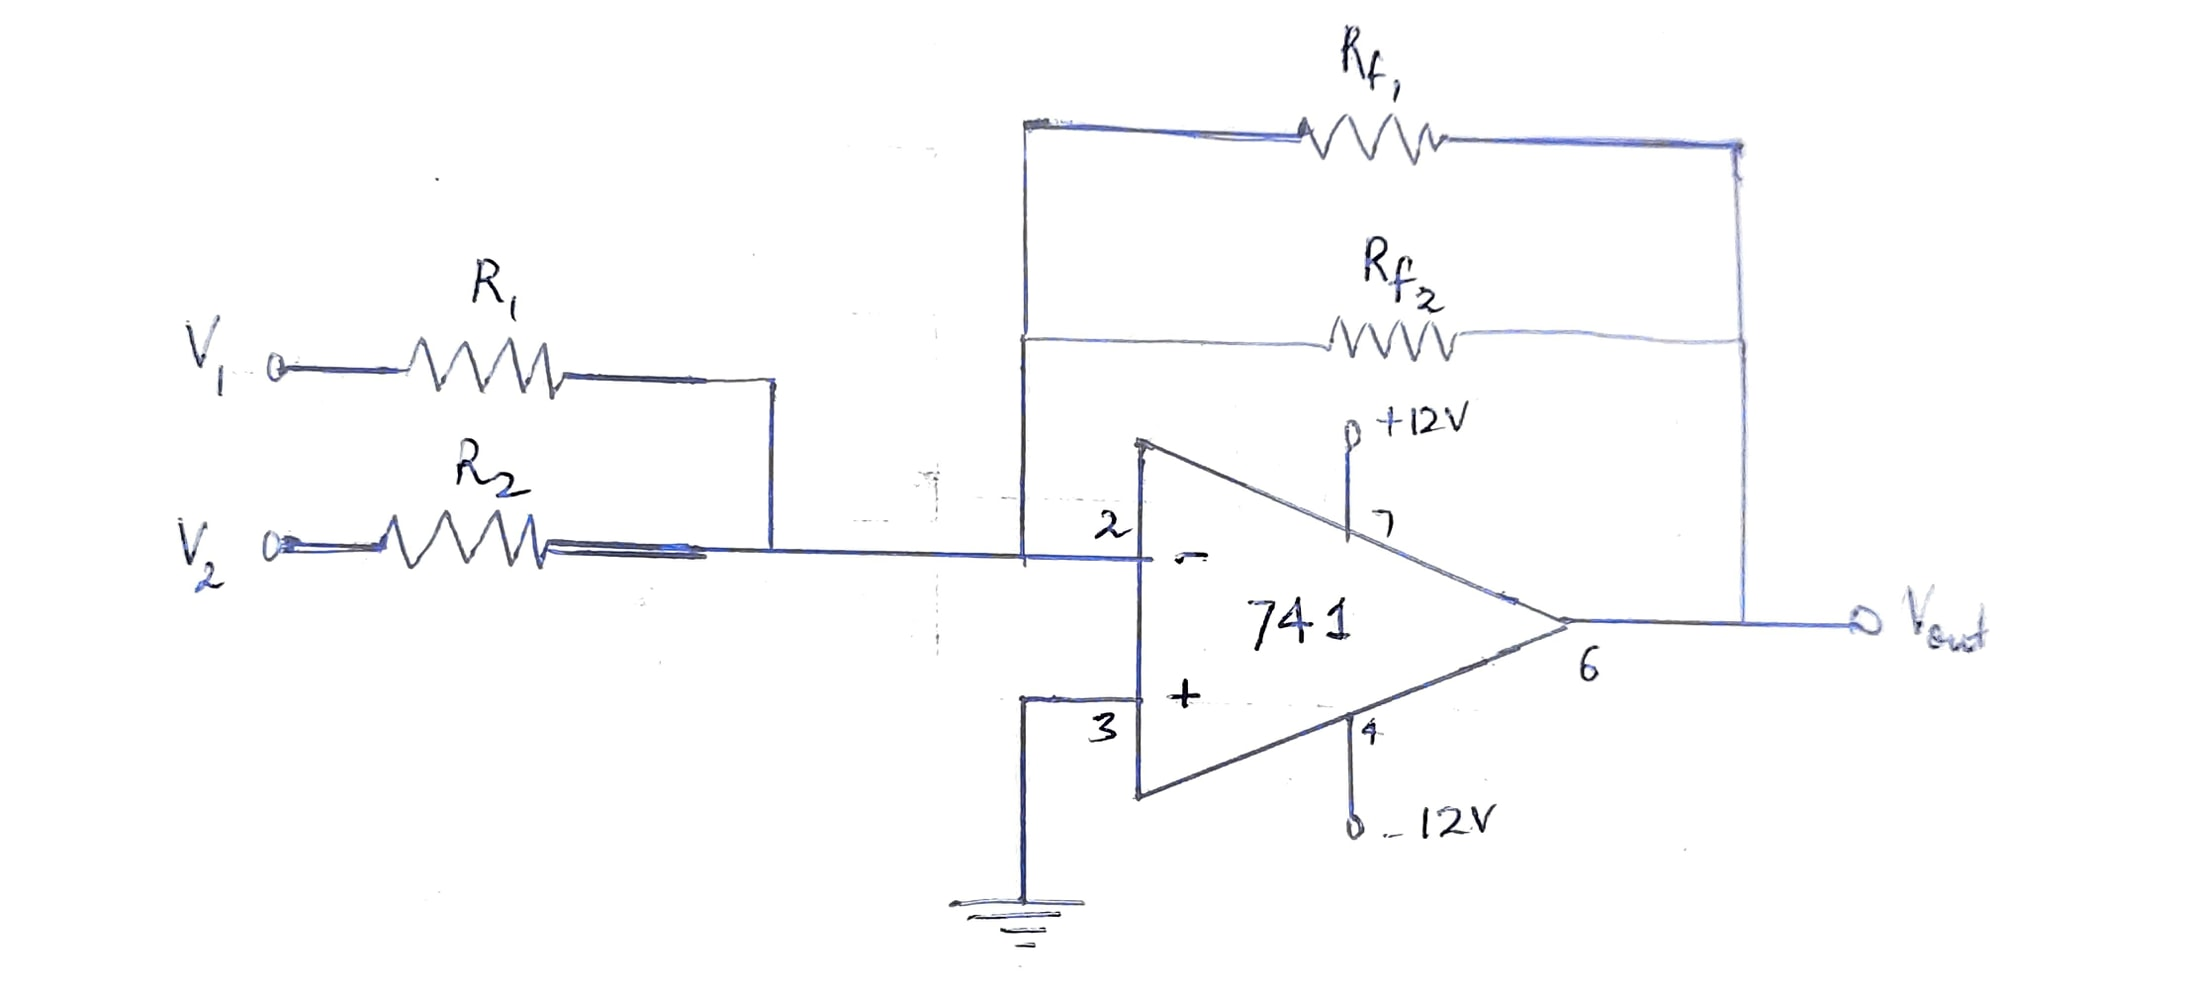
\includegraphics[scale = 0.2]{OPAMP Config/averaging.jpg}
\end{center}
\begin{center}
    \textbf{Averaging Amplifier Circuit}
\end{center}
\noindent Note that $R_{f_1} = R_{f_2}$
\section{Observations}
\noindent \textbf{\emph{For Inverting and Non-inverting Amplifier Circuits:}}
\begin{enumerate}
    \item $R_{f_1} = \SI{9.98}{k\ohm}$, $R_{f_2} = \SI{17.55}{k\ohm}$
    \item $R_3 = \SI{0.985}{k\ohm}$
    \item $R_i = \SI{0.997}{k\ohm}$
\end{enumerate}
\textbf{\emph{For Summing, Difference and Averaging Amplifier Circuits:}}
\begin{enumerate}
    \item $R_1 = \SI{9.92}{k\ohm}$
    \item $R_2 = \SI{10.06}{k\ohm}$
    \item $R_3 = \SI{9.88}{k\ohm}$
    \item $R_f = \SI{10.02}{k\ohm}$
    \item $R_{f_{avg}} = R_3 || R_f = \SI{4.975}{k\ohm}$
\end{enumerate}
\clearpage
\begin{center}
    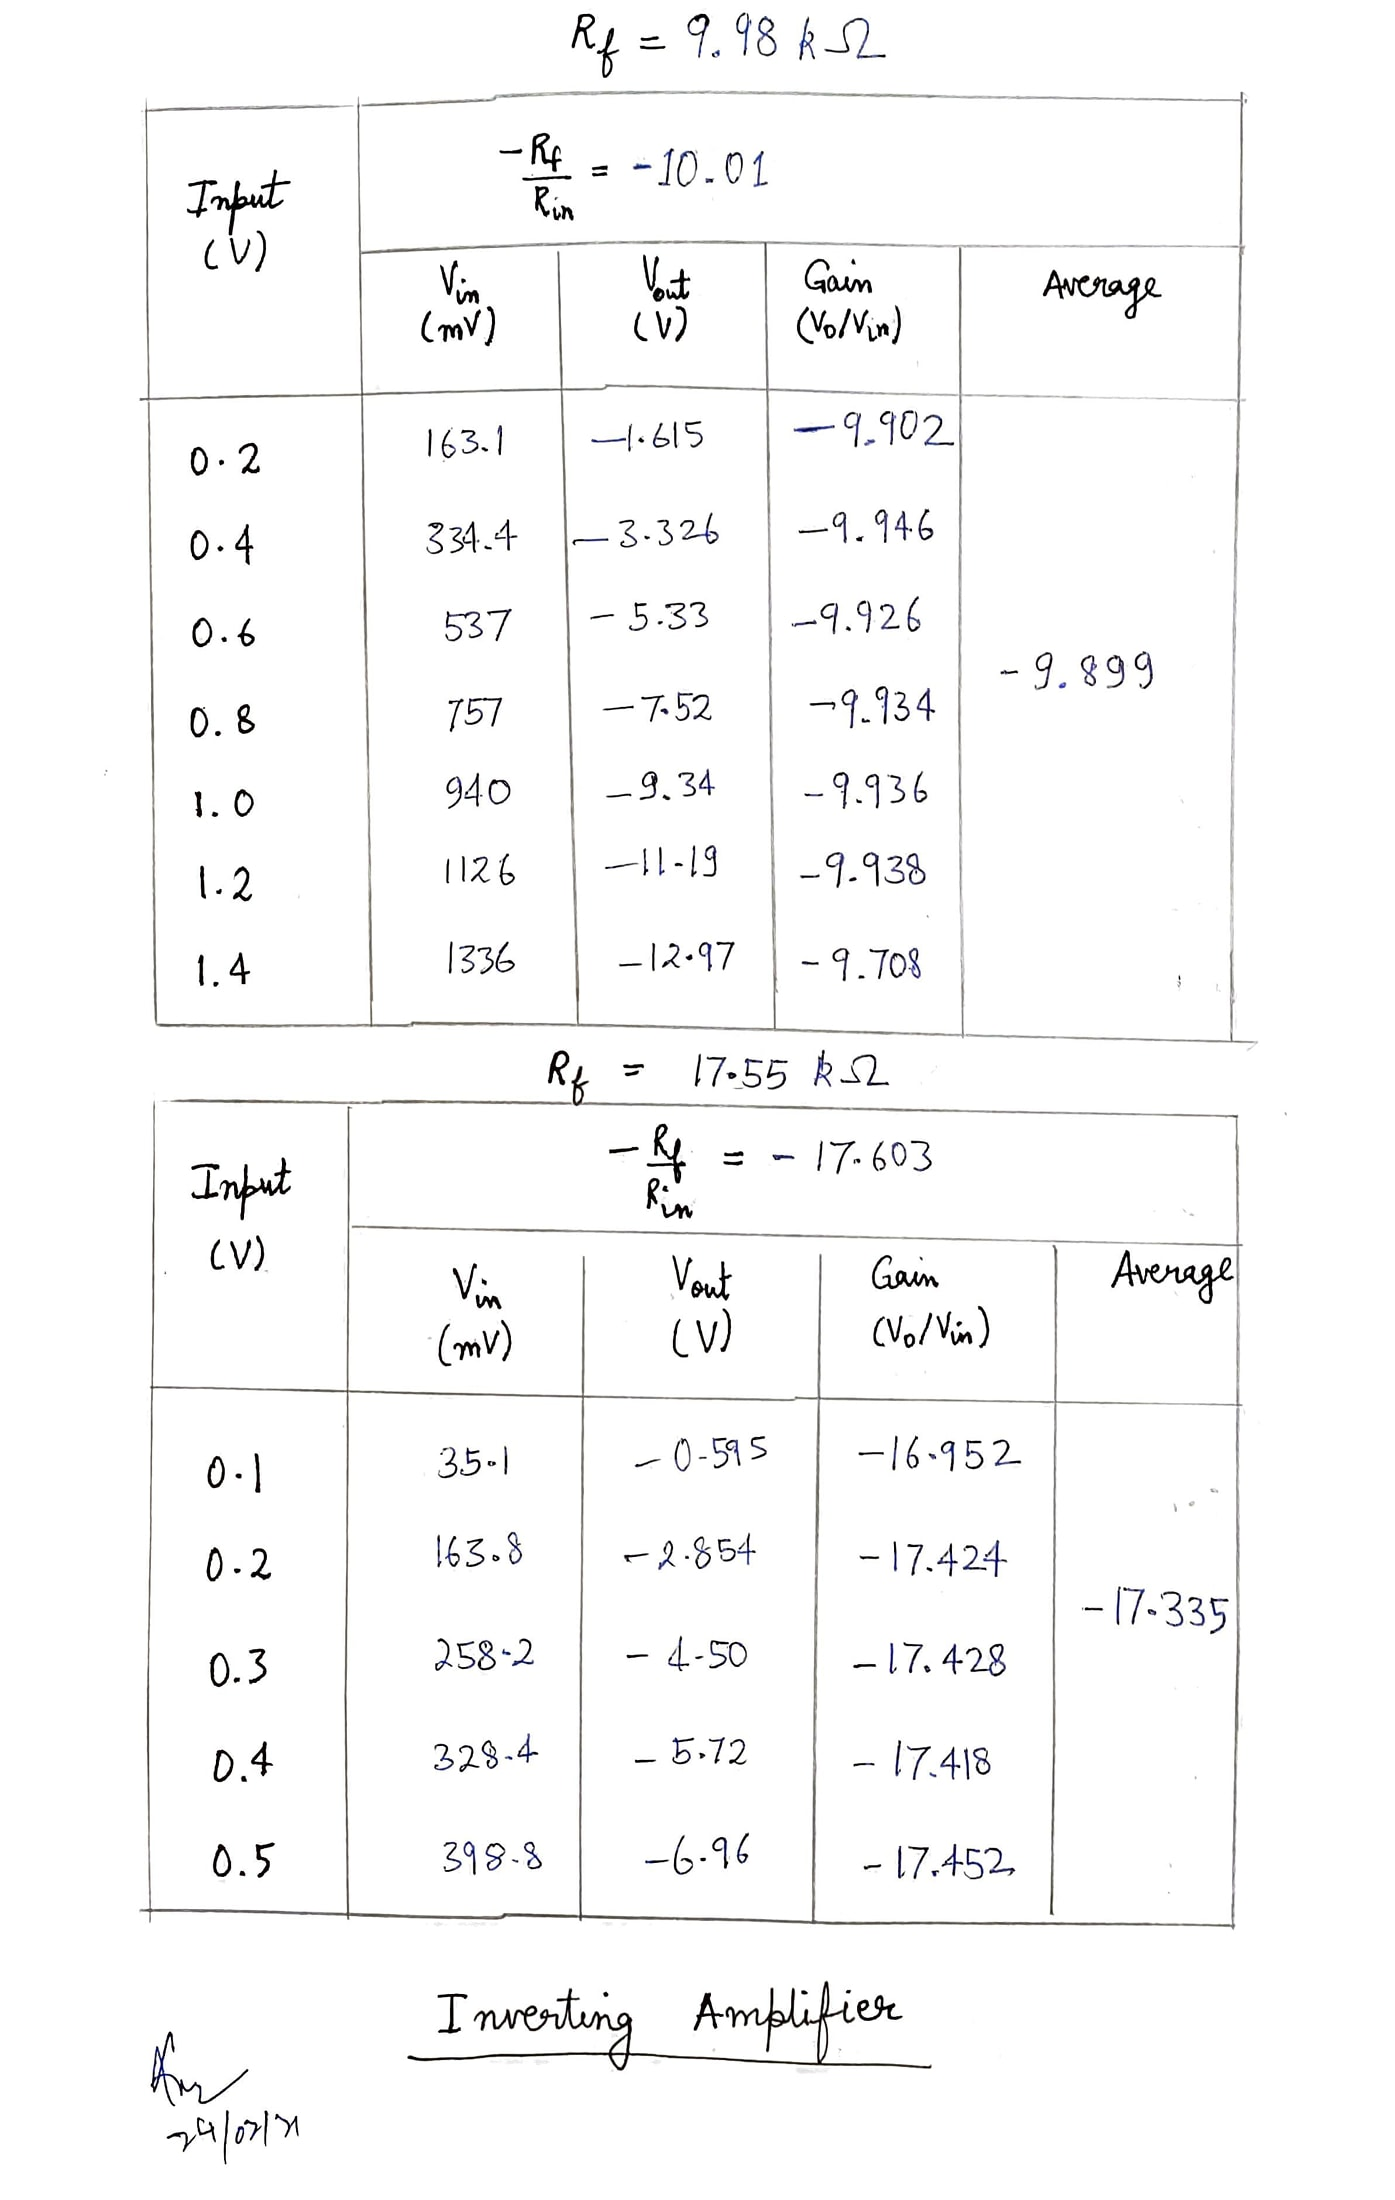
\includegraphics[scale = 0.25]{OPAMP Config/invamp.jpg}
\end{center}
\clearpage
\begin{center}
    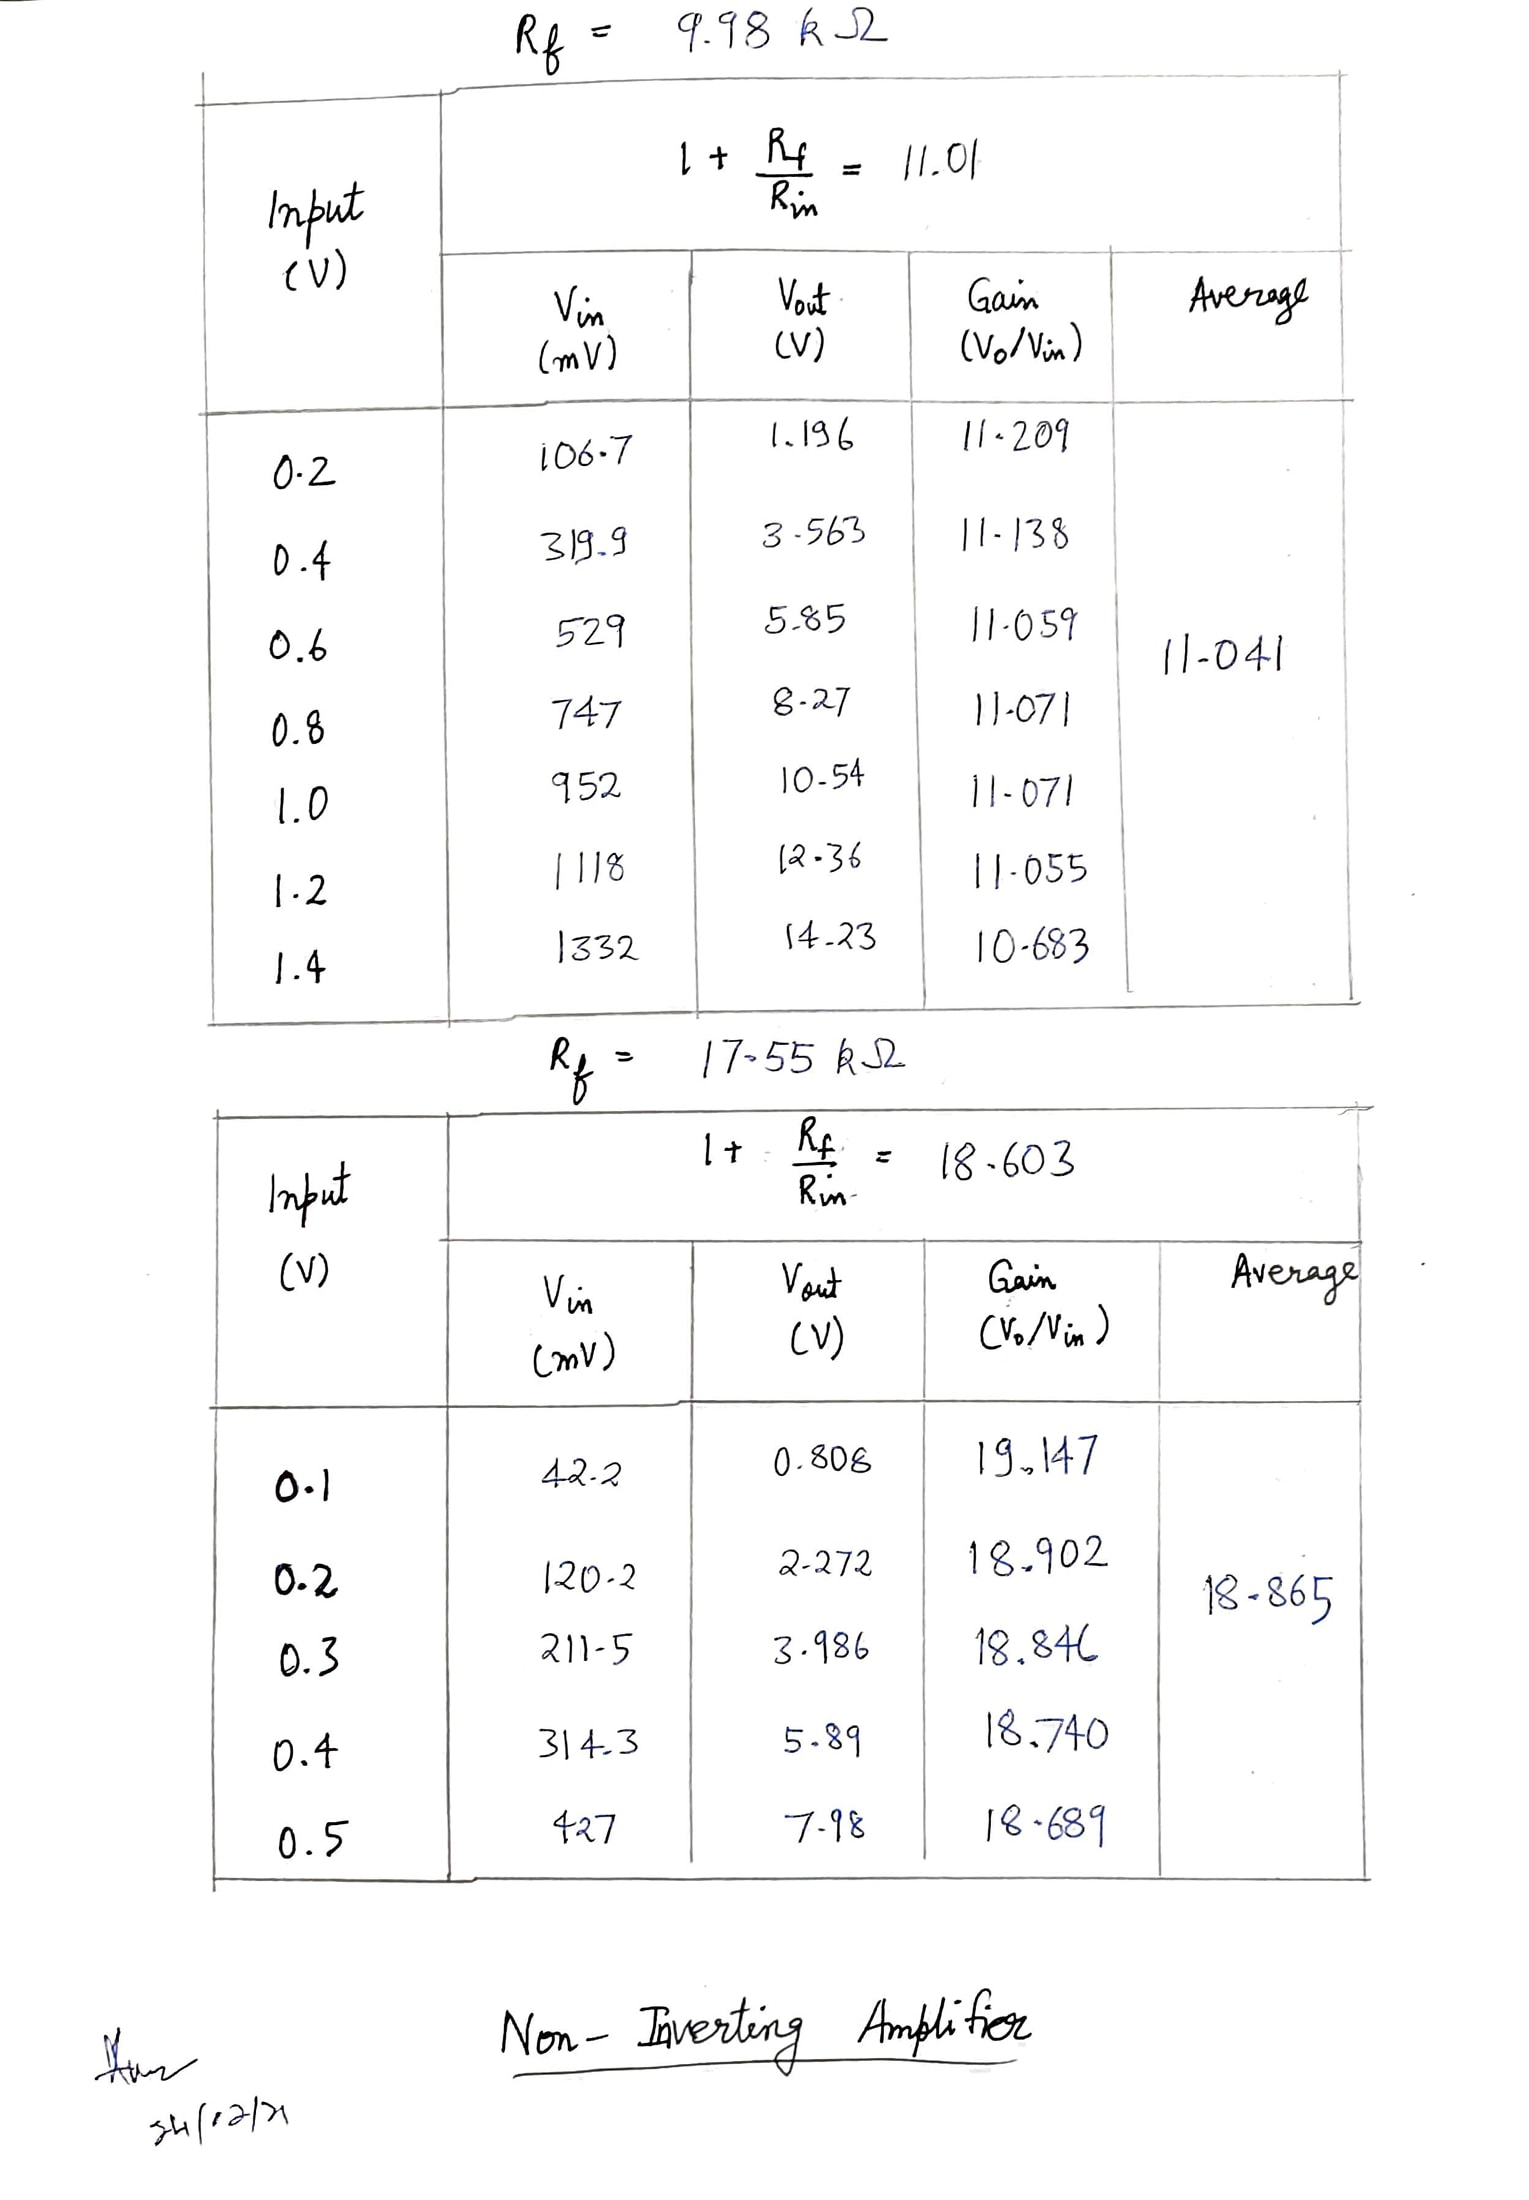
\includegraphics[scale = 0.25]{OPAMP Config/noninvamp.jpg}
\end{center}
\clearpage
\begin{center}
    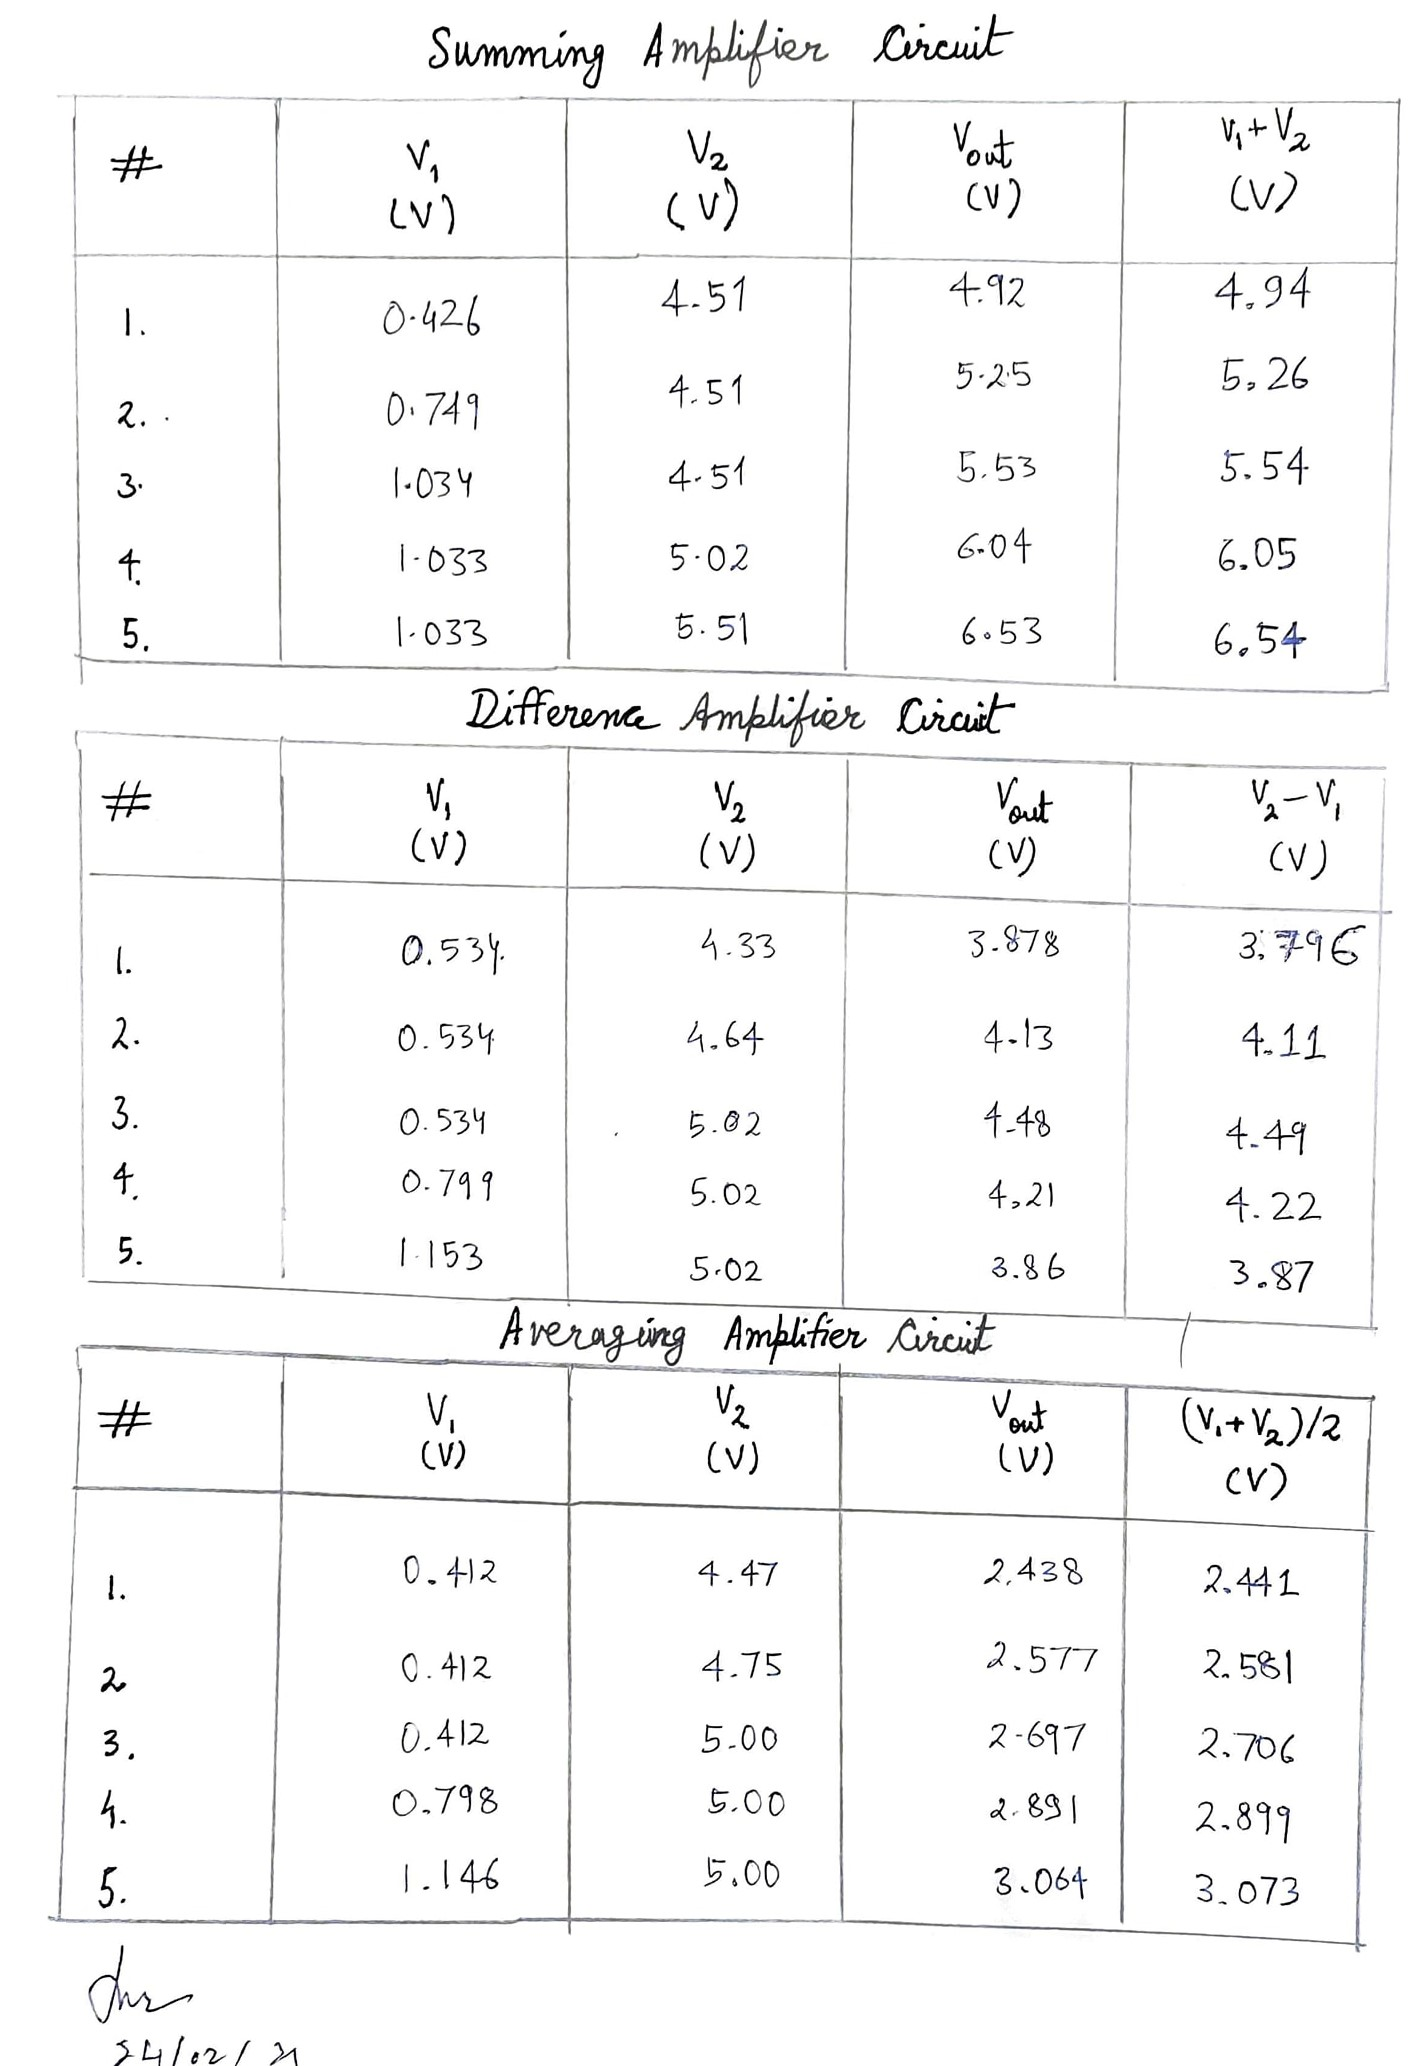
\includegraphics[scale = 0.4]{OPAMP Config/sumdiffavg (2).jpg}
\end{center}
\clearpage
\section{Graphs}
\begin{center}
    \textbf{Inverting Amplifier}
\end{center}
\begin{center}
    $R_f = \SI{9.98}{k\ohm}$
\end{center}
\begin{center}
    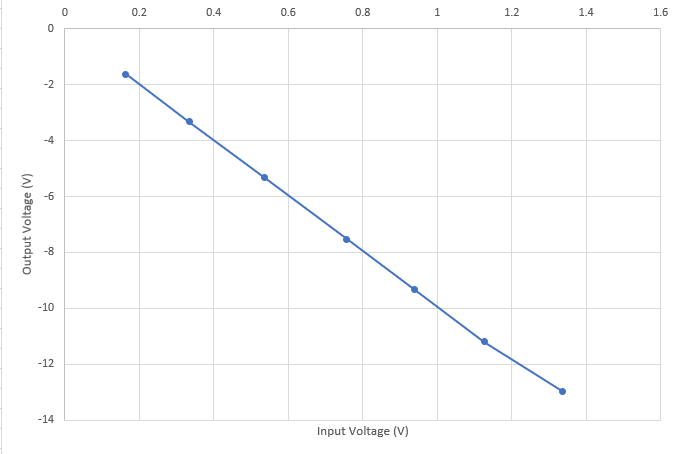
\includegraphics[scale = 0.7]{OPAMP Config/invampf1.png}
\end{center}
\begin{center}
    $R_f = \SI{17.55}{k\ohm}$
\end{center}
\begin{center}
    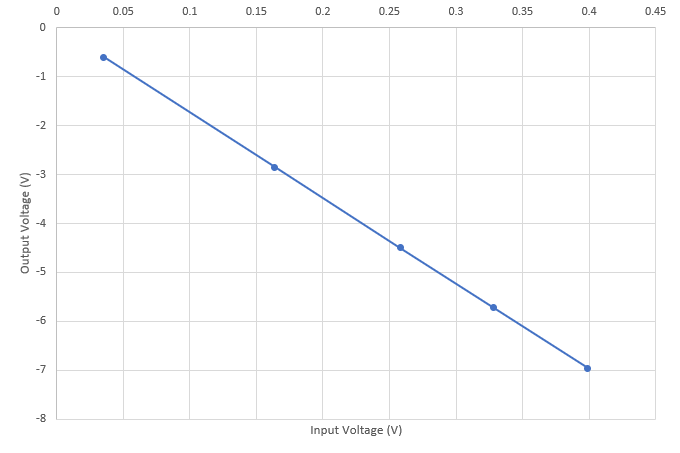
\includegraphics[scale = 0.7]{OPAMP Config/invampf2.png}
\end{center}
\begin{center}
    \textbf{Non-inverting Amplifier}
\end{center}
\begin{center}
    $R_f = \SI{9.98}{k\ohm}$
\end{center}
\begin{center}
    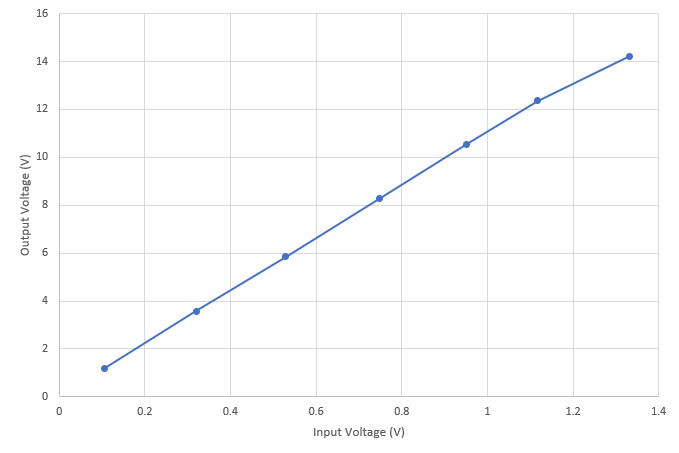
\includegraphics[scale = 0.7]{OPAMP Config/noninvampf1.png}
\end{center}
\begin{center}
    $R_f = \SI{17.55}{k\ohm}$
\end{center}
\begin{center}
    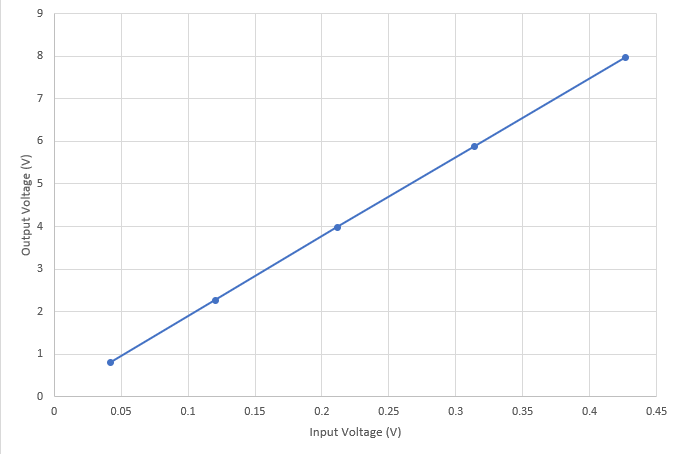
\includegraphics[scale = 0.7]{OPAMP Config/noninvampf2.png}
\end{center}
\clearpage
\section{Results}
\begin{enumerate}
    \item The inverting amplifier accepts an input voltage signal and increases the output voltage signal by a certain constant factor with a opposite sign.
    \item The non-inverting amplifier accepts an input voltage signal and increases the output voltage signal by a certain constant factor with no change in sign.
    \item The summing amplifier accepts two input voltage signals and the output voltage signal is found to be equal to the summation of those two.
    \item The difference amplifier accepts two input voltage signals and the output voltage signal is found to be equal to the difference of those two.
    \item The averaging amplifier accepts two input signals and the output output voltage signal is found to be equal to the average of those two.
\end{enumerate}
\section{Discussions}
\begin{enumerate}
    \item The inverting amplifier amplifies the input voltage signal by a certain constant factor which is called \textbf{\emph{gain}} and changes the sign too. This change in sign can be attributed to the inversion of the output signal with respect to the input signal as it is $\pi$ degrees out of phase.
    \item On the other hand, the output signal in non-inverting amplifier is in the same phase as that of input signal so there is no change in sign.
    \item We can note that the Gain as calculated from the formulae is not exactly equal to the gain that is calculated experimentally. Therefore there is some error. This error can be attributed to various factors from imperfections in the Op-Amp IC741, capacitance of breadboard and fluctuations caused my nearby surroundings. These things can collectively called as noises in the signal.
    \item Taking a look at the formulae, we can deduce that practically no current enters the Op-Amp input terminals. In fact, in other words, there is a virtual ground at the junction of input signal and feedback loop.
    \item The summing amplifier works in a similar fashion to that of the inverting amplifier with multiple input signals. Similarly the difference and averaging amplifiers are also based on similar modification of input signals.
    \item After careful observation of the inverting and non-inverting amplifier curves, we can deduce that the Op-Amp will not have infinite gain, rather the output will plateau after some time. The plateaued value can be linked to the biasing voltage that is applied across the Op-Amp.
    \item We can use the Op-Amp to construct many linear combination of inputs from which can a desired output can be obtained.
    \item The IC741 is a widely used component but we can use some other Op-Amp with a better slew rate.
    
\end{enumerate}
\section{Error Analysis}
\begin{enumerate}
    \item For \textbf{Inverting Amplifier}, with $R_f = \SI{9.98}{k\ohm}$, the theoretical value is $-10.01$ and experimental value is $-9.899$. Therefore the error is given by
    \begin{center}
        Percentage error = $\dfrac{-10.01-(-9.899)}{-10.01} \times 100 \% = 1.11\%$
    \end{center}
    \item For \textbf{Inverting Amplifier}, with $R_f = \SI{17.55}{k\ohm}$, the theoretical value is $-17.603$ and experimental value is $-17.335$. Therefore the error is given by
    \begin{center}
        Percentage error = $\dfrac{-17.603-(-17.335)}{-17.603} \times 100 \% = 1.52\%$
    \end{center}
    \item For \textbf{Non-inverting Amplifier}, with $R_f = \SI{9.98}{k\ohm}$, the theoretical value is $11.01$ and experimental value is $11.041$. Therefore the error is given by
    \begin{center}
        Percentage error = $\dfrac{11.01-11.041}{11.01} \times 100 \% = -0.28\%$
    \end{center}
    \item For \textbf{Non-inverting Amplifier}, with $R_f = \SI{17.55}{k\ohm}$, the theoretical value is $18.603$ and experimental value is $18.865$. Therefore the error is given by
    \begin{center}
        Percentage error = $\dfrac{18.603-18.865}{18.603} \times 100 \% = -1.41\%$
    \end{center}
\end{enumerate}
\section{Conclusion}
\begin{enumerate}
    \item All components of the circuit performed according to the expectations. 
    \item The sources of error are discussed and error analysis reveals that errors were quite small.
\end{enumerate}